% don't remove the following lines, and edit the definition of \main if needed
\documentclass[../report.tex]{subfiles}
\providecommand{\main}{..}
\IfEq{\jobname}{\currfilebase}{\AtEndDocument{\biblio}}{}
% until here

\newcommand{\sigv}{\langle \sigma v_{\rm{rel}} \rangle}
\newcommand{\MET}{\slashed{E}_T}
\newcommand{\mDM}{m_{\rm{DM}}}
\newcommand{\mmed}{M_{\rm{med}}}
\newcommand{\mMed}{M_{\rm{med}}}
\newcommand{\gDM}{\ensuremath{g_{\mathrm{DM}}}}
\newcommand{\gq}{\ensuremath{g_q}}
\newcommand{\gSM}{\ensuremath{g_q}}
\newcommand{\gf}{\ensuremath{g_f}}

\newcommand{\ifb}{\rm{fb}^{-1}}

\newcommand{\mA}{M_{A}}
\newcommand{\GamA}{\Gamma_{A}}

\begin{document}

\section{Dark Matter}
\label{sec:BSM-DM}

%The majority of matter in the observable Universe is dark, thus far unobservable to all experimental probes save for a handful of gravitational hallmarks left indelibly in the dynamics of galaxies and the Universe as a whole.  These hallmarks only reveal the large-scale dynamics of this unknown matter, leaving the discovery of the small-scale, microscopic, origins of dark matter (DM) as a primary objective in the future exploration of the particle world.

%If DM is composed of massive objects, its fundamental constituents could range in mass from truly microscopic particles evading current collider energies to macroscopic objects such as primordial black holes. Consequently, particle physics plays an important role in the systematic exploration of the nature of DM and its interactions, complementing experiments and observations from astroparticle physics (see Sect.~\ref{chapDM}). 

For an introduction to dark matter (DM) and a general study of its experimental consequences, see Chapter~\ref{chap:dm}. This section presents the ways in which the nature of DM and its interactions can be probed at future colliders, complementing experiments and observations from astroparticle physics. 

The thermal freeze-out mechanism provides a cosmological clue for the generation of the observed DM density, suggesting that DM particles have masses in the range from multi-keV to about 100~TeV, and couplings to SM particles of comparable or weaker strength than EW interactions. High-energy colliders could produce DM particles within this mass range in controlled conditions. The main signature at colliders is the missing transverse momentum carried by the DM particle, which remains invisible to detectors due to the presumed weak strength of its interaction with SM particles. If the DM particle is lighter than $m_h/2$ and it is coupled to the Higgs, an interesting exploration channel is the invisible Higgs decay width (see Chapters~\ref{chap:ew} and \ref{chap:dm}). An alternative signature is the detection of the mediator particles whose exchange may be responsible for the annihilation processes that determine the DM particle abundance. Mediators can lead to a variety of collider signatures in visible channels, although their discovery would not provide evidence for DM until invisible channels are identified as well.
 
There are many possible thermal freeze-out scenarios, each with their own unique experimental signals. Here we present only some interesting examples of heavy DM particles and discuss the prospects for their searches at future colliders. The case of light DM particles is addressed in Sect.~\ref{sec:BSM-FIPs} and non-collider searches for DM are discussed in Chapter~\ref{chap:dm}.

\subsection{Higgsinos and Winos}

The most straightforward example of a DM thermal relic is a massive particle with EW gauge interactions only. Of special interest are the cases of spin-1/2 particles transforming as doublets or triplets under SU(2) symmetry, which are usually referred to as Higgsino and Wino respectively. Although this terminology is borrowed from SUSY, these examples should be regarded as standalone DM models.

A summary of the reach of future colliders for Higgsinos and Winos is presented in Fig.~\ref{fig:HiggsinoWino} (for a more detailed discussion of the relevant collider signatures, see Sect.~\ref{sec:BSM-SUSY-weak}).  
%The minimal one-loop predicted neutral-charged mass splitting is assumed, however in the presence of additional heavy states the mass splitting can be modified.  In such cases, fine-tuned additional contributions could be chosen to modify the collider phenomenology and perhaps obscure the particles from view.  
A study of the preferred mass range from thermal freeze-out can be found in \cite{Krall:2017xij}.  Current direct detection limits are not shown as, for a pure Higgsino with a small inelastic splitting, the spin-independent cross-section is well below the irreducible neutrino background.  For the Wino the cross-section is above the neutrino background, but only by less than an order of magnitude \cite{Chen:2018uqz}.  DARWIN, a future direct detection experiment, is expected to probe the Wino scenario up to masses of $2\substack{+3 \\ -1}$ TeV, where the large error reflects the theoretical uncertainties on the Wino-proton cross-section~\cite{Chen:2018uqz}.  This projection is shown in Fig.~\ref{fig:HiggsinoWino}. Current indirect detection limits were taken from \cite{Krall:2017xij}, which compiled both FERMI and H.E.S.S. telescope constraints.  Note that the indirect detection constraints are subject to large systematic uncertainties from halo-shape modelling.  These uncertainties are not reflected in the bars shown in Fig.~\ref{fig:HiggsinoWino} and should be kept in mind when comparing with collider searches. 

The reach for disappearing track searches at \HLLHC, \HELHC and \FCChh is taken from \cite{CidVidal:2018eel}, while the result for low-energy \FCChh is obtained with a simple extrapolation. The reach for Higgsinos at \FCCeh is taken from Vol.~1 of the FCC CDR \cite{Abada:2019lih}, while the \FCCeh reach for Winos was provided in a private communication by the  collaboration. Due to the cleanliness of the interactions, direct searches at lepton colliders typically come close to the kinematical limit (shown in blue in Fig.~\ref{fig:HiggsinoWino}), but do not surpass it.  On the other hand, the sensitivity to the EW parameters $W$ and $Y$ allows for a reach that can extend beyond the kinematic limit, albeit in an indirect manner.  These constraints, shown in grey, are calculated using the formulae of~\cite{DiLuzio:2018jwd} updated with the sensitivity reported in the ECFA Higgs report \cite{deBlas:2019rxi}. It is important to remark that \FCChh can conclusively test the hypothesis of thermal DM for both the Higgsino and Wino scenarios, while \CLIC can cover the Higgsino case. These results were obtained assuming the EW one-loop neutral-charged mass splitting (see Sect.~\ref{sec:BSM-SUSY-weak}). \FCChh searches could become ineffective under the special circumstances of heavy-particle contributions that accidentally cancel the loop-induced mass splitting.

\begin{figure}[htb]
%\begin{figure}[t]
    \centering
    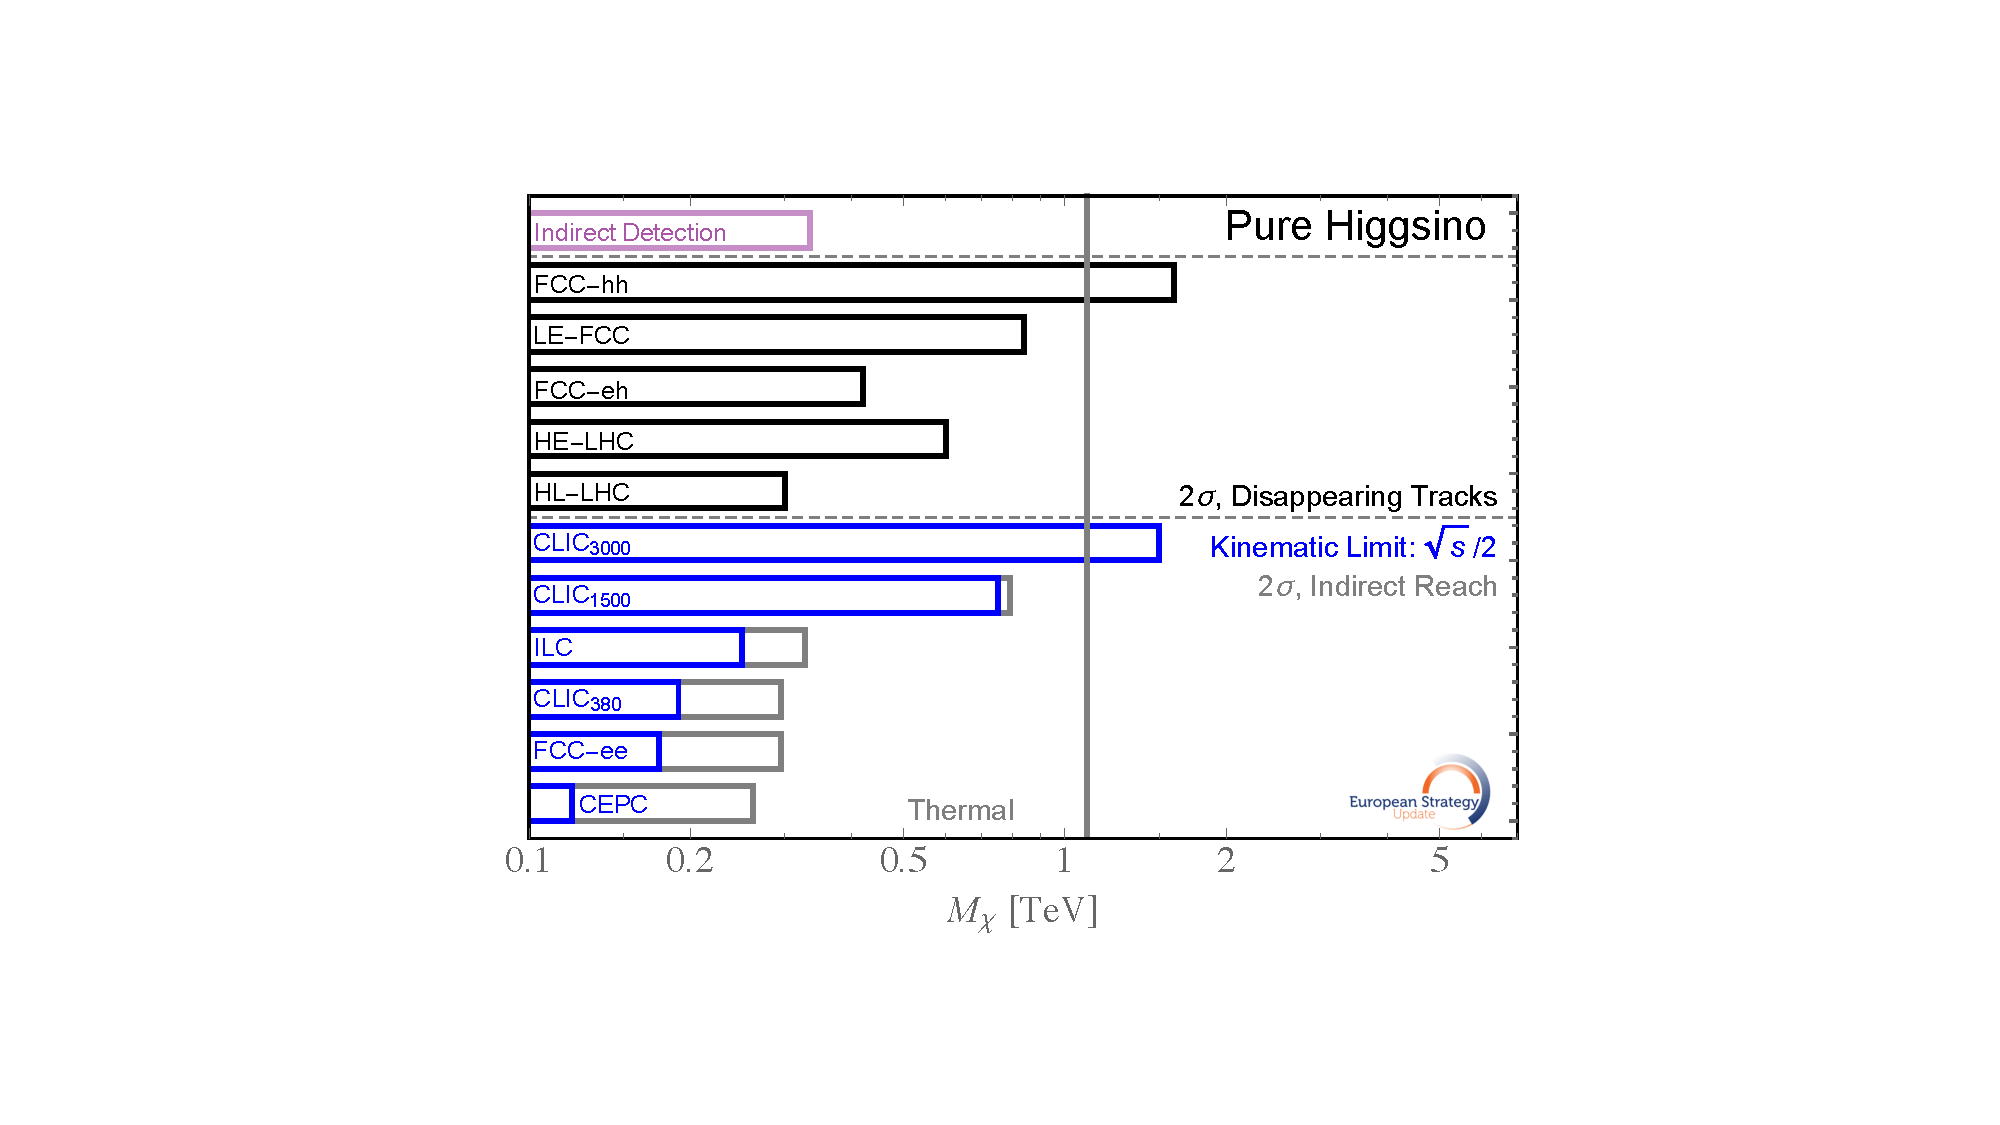
\includegraphics[width=0.48\textwidth]{\main/BSM/DM/plots_DM/Higgsino}
   ~ 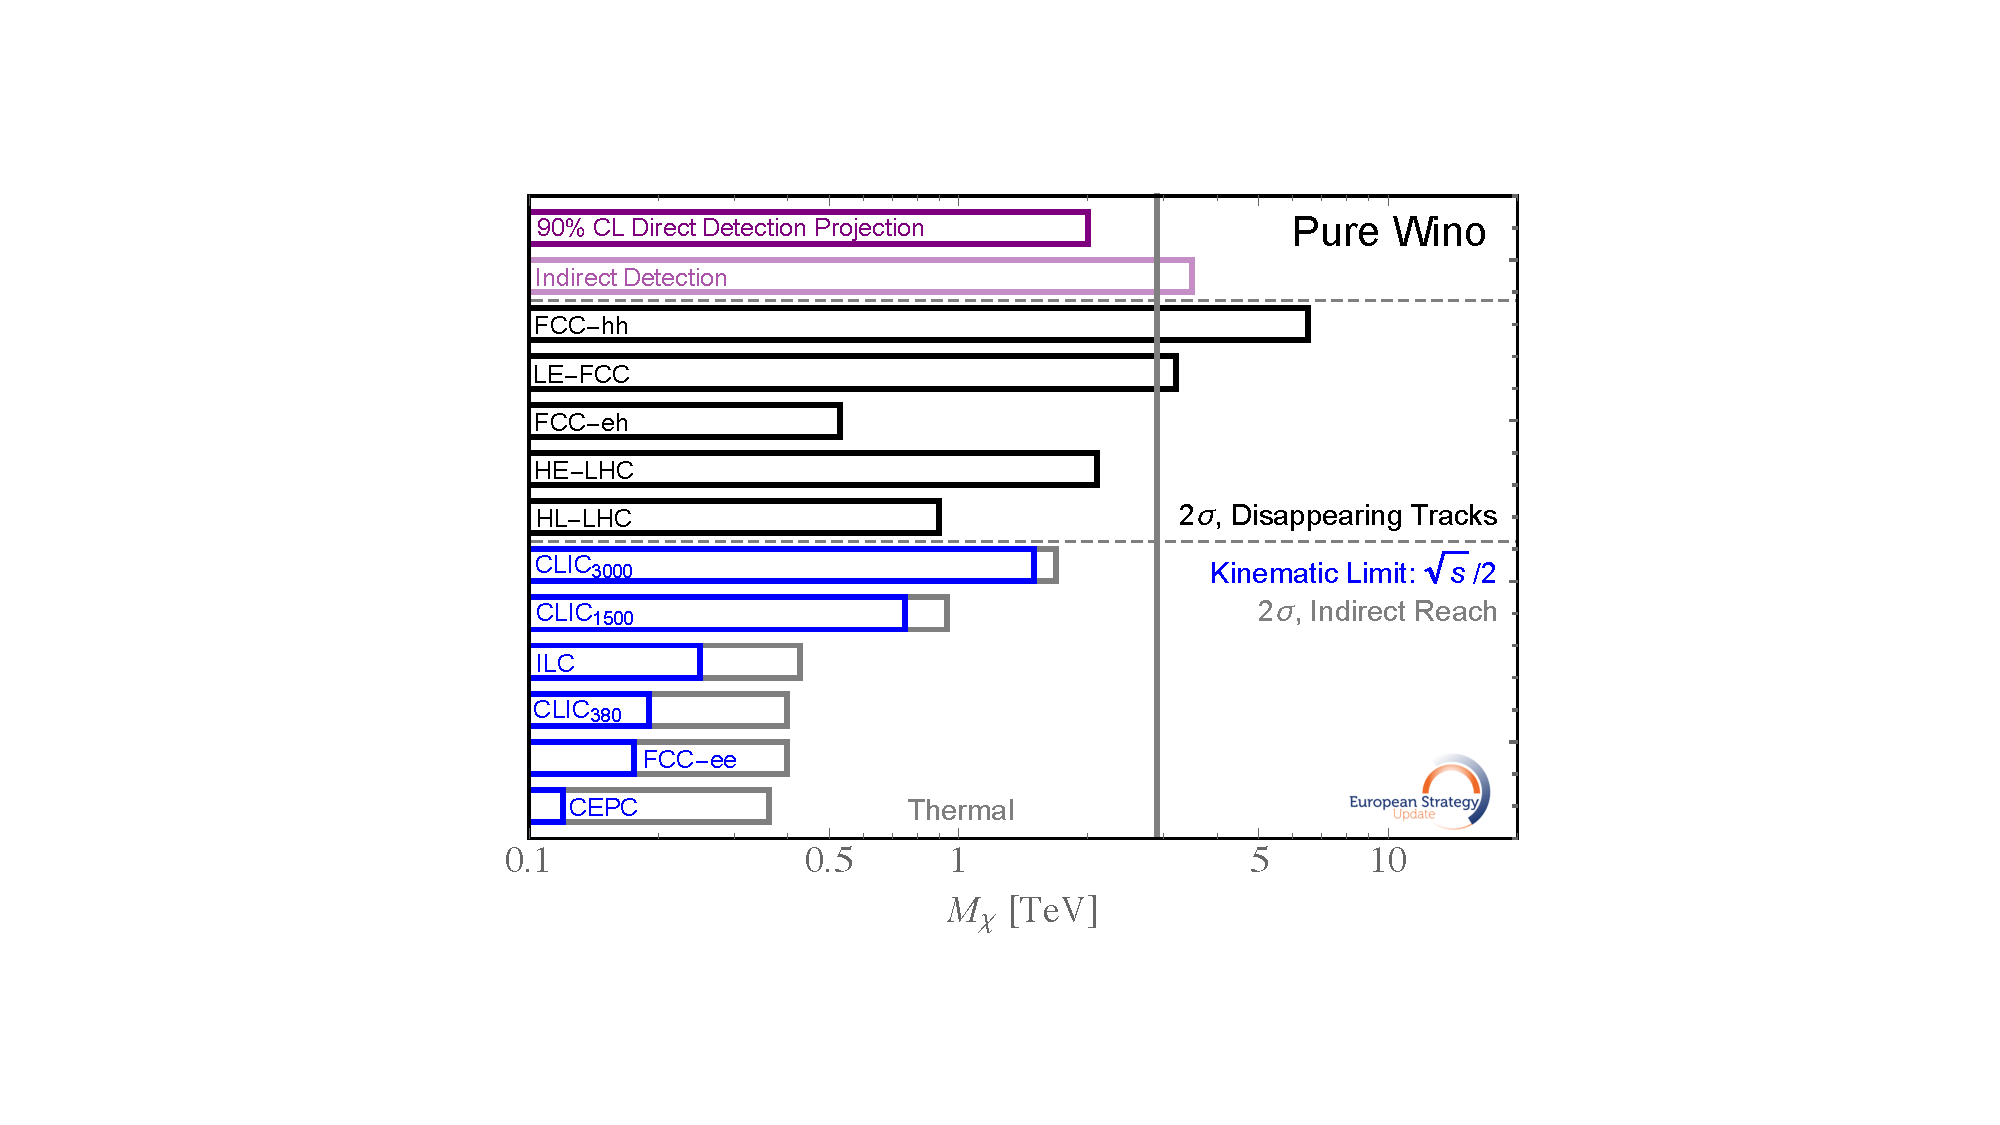
\includegraphics[width=0.48\textwidth]{\main/BSM/DM/plots_DM/Wino}
    \caption{Summary of $2\sigma$ sensitivity reach to pure Higgsinos and Winos at future colliders. Current indirect DM detection constraints (which suffer from unknown halo-modelling uncertainties) and projections for future direct DM detection (which suffer from uncertainties on the Wino-nucleon cross-section) are also indicated. The vertical line shows the mass corresponding to DM thermal relic.}
    \label{fig:HiggsinoWino}
\end{figure}

\subsection{Simplified Models: axial vector and scalar mediators}

Simplified DM Models are a schematic way to parametrise classes of theories without committing to specific dynamical constructions or introducing too many unknown parameters. The Simplified Models considered here introduce one DM particle and one mediator, and their free parameters are the masses of these two particles and the coupling constants of the interactions mediator/DM and mediator/SM particles. The mediator can be either a SM particle itself (e.g. the Higgs or the $Z$ boson) or a new BSM particle. Depending on the nature of the DM particle and the mediator, one can construct a large variety of Simplified Models and here two representative examples~\cite{Abercrombie:2015wmb} are chosen.

In both cases, the DM particle is a massive Dirac fermion ($\chi$). In the first example, the mediator is a spin-1 particle ($Z^\prime$) coupled to an axial-vector current in the Lagrangian as $-Z^\prime_\mu (g_{\rm DM} \, \bar{\chi}\gamma^{\mu}\gamma_5\chi + g_f \sum_{f}  \bar{f}\gamma^{\mu}\gamma_5f )$, where $f$ are SM fermions. This model is particularly interesting for collider searches because the reach of direct DM searches is limited, as the  interaction in the non-relativistic limit is purely spin-dependent.  In the second example, the mediator is a spin-0 particle ($\phi$) with interactions $\phi (g_{\rm DM}\, \bar{\chi}\chi-  g_f   \sum_{f} y_f \bar f f /\sqrt{2})$. This model can serve as a prototype for various extensions of the SM involving enlarged Higgs sectors.

In Fig.~\ref{fig:AxialVectorScalar} a compilation of future collider sensitivities to the two Simplified Models under consideration, with a choice of couplings of ($g_{\rm f}=0.25$, $g_{\rm DM}=1.0$) for the axial-vector model and ($g_{\rm f}=1.0$, $g_{\rm DM}=1.0$) for the scalar model, are shown. The reach of collider experiments to this kind of models is strongly dependent on the choice of couplings. As an example, the sensitivity of dijet and monojet searches decreases significantly with decreased quark couplings: with 36 fb$^{-1}$ of LHC data~\cite{Aaboud:2019yqu} and assuming a DM mass of 300 GeV and $g_{\rm DM}=1.0$, the limits from dijet searches on the axial-vector mediator mass decrease from 2.6 TeV for a quark coupling of $g_{\rm q}=0.25$ to 900 GeV for $g_{\rm q}=0.1$, while the monojet limits decrease from 1.6 TeV ($g_{\rm q}=0.25$) to 1 TeV ($g_{\rm q}=0.1$). 

The mono-photon constraints at lepton colliders result from the mediator coupling to leptons, whereas at hadron colliders only the quark couplings are relevant.  As a result, the two cases cannot be compared like-for-like, although the results illustrate the relevant strengths for exploring the dark sector in a broad sense.  Furthermore, mono-photon constraints apply in a general EFT context, hence additional complementary coupling-dependent constraints, such as on four-electron interactions, may be relevant. 

Constraints for \HLLHC and \HELHC are taken from \cite{CidVidal:2018eel, Haisch:2018bby}.  The \FCChh monojet constraints for the axial-vector model are estimated using the collider reach tool, with results consistent with the analysis performed in \cite{Abada:2019lih}. Estimates for \FCChh, in the case of the scalar model, are taken from~\cite{Harris:2015kda}.  Estimates for low-energy FCC-hh (LE-FCC) are generated from the collider reach tool alone. Complementary dijet-resonance constraints for the axial-vector model are taken from \cite{Golling:2016gvc,Harris:2015kda}.  For the lepton colliders, the \CLIC monophoton estimates were provided privately by the CLIC collaboration and all other lepton collider estimates are taken from \cite{Habermehl:2018yul}. For CEPC estimates, without considering systematic uncertainties, see~\cite{Liu:2019ogn}.
It is clear from these estimates that future colliders can provide sensitive probes of DM, potentially revealing evidence for invisible particle production, even for very massive mediators. 

\begin{figure}[htb]
    \centering
    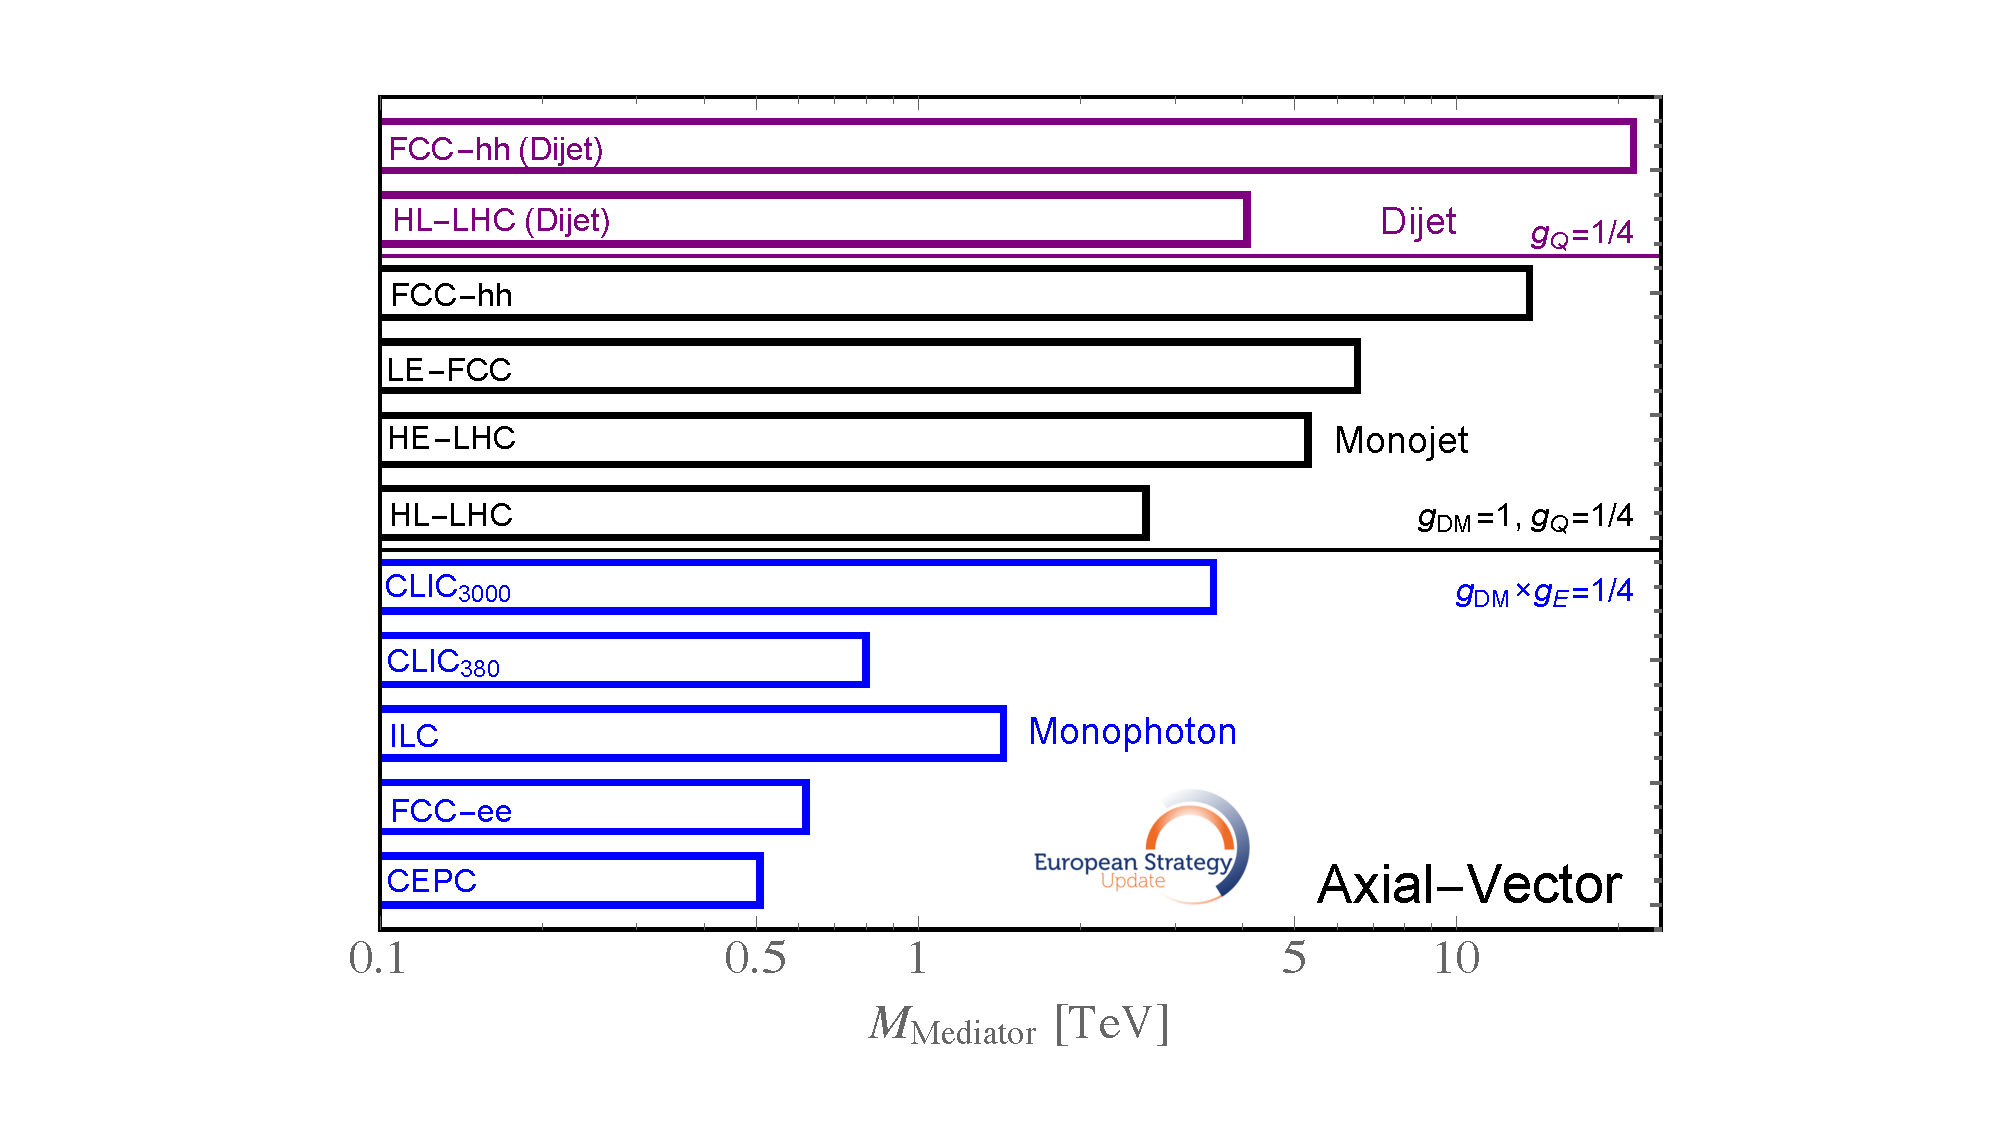
\includegraphics[width=0.48\textwidth]{\main/BSM/DM/plots_DM/AxialVector}
    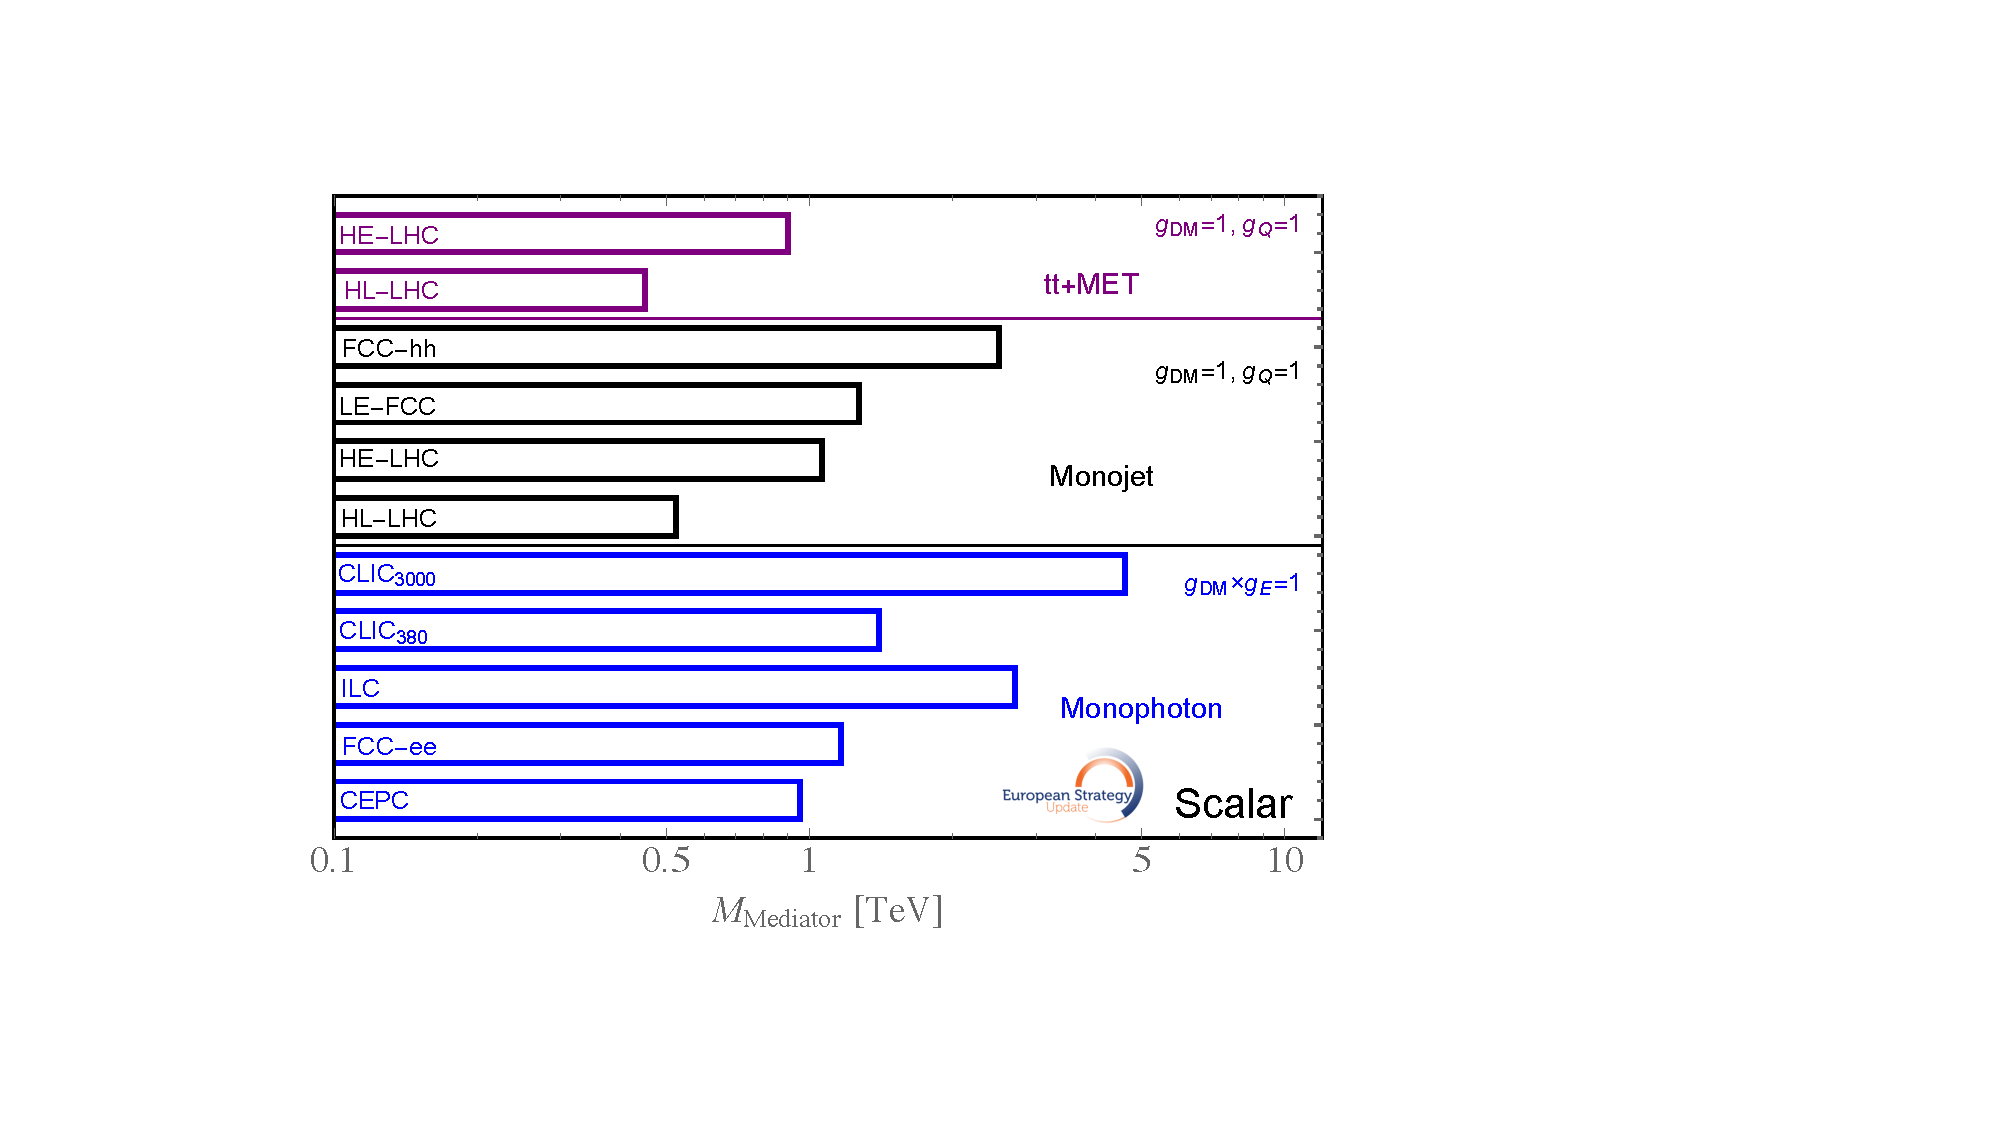
\includegraphics[width=0.48\textwidth]{\main/BSM/DM/plots_DM/Scalar}
    
\caption{Summary of $2\,\sigma$ sensitivity to axial-vector and scalar simplified models at future colliders for a DM mass of $M_{\rm{DM}}=1$ GeV and for the couplings shown in the figure. References and details on the estimates included in these plots can be found in the text. }
    \label{fig:AxialVectorScalar}
\end{figure}

Searches at high-energy hadron colliders have the best reach for the visible decays of multi-TeV mediator particles. Going beyond the \HLLHC reach for those same resonances in the mass region between 10 GeV and 1 TeV is still possible with an increased dataset at hadron colliders (see Sect.~\ref{sec:BSM-FIPs} and e.g.\ Ref.~\cite{Curtin:2014cca}), but it is inherently more challenging than for lepton colliders. It is often the case that signatures of sub-TeV resonances at hadron colliders are indistinguishable from those of their high-rate backgrounds, especially considering the impact of simultaneous $pp$ interactions on searches for hadronically decaying resonances at high-luminosity hadron colliders. Since it is generally not possible to record all events in their entirety for further analysis, as doing so would saturate the experiment data-acquisition and trigger systems, maintaining the sensitivity for sub-TeV resonances at hadron colliders requires the employment of specific data-taking and analysis techniques~\cite{2018arXiv180208640A} (see also Chapter~\ref{chap:inst}).

The discovery of invisible particles at a collider experiment does not imply that those invisible particles constitute the cosmological dark matter; for that, it would be necessary to compare collider results to direct and indirect detection experiment, as well as to astrophysical observations (e.g.\ the dark matter relic density). The comparison of the sensitivity of experiments at future colliders and direct/indirect detection experiments searching for dark matter for the models in this section can be found in Chapter~\ref{chap:dm}. 

\end{document}

